%!TeX root = main.tex
% TODO; wie darf ich einen meromorphen verändern, (das P verändern) ohne das
% sich effektiv was ändert?
% TODO: \cM = \cM_K ... replace
% TODO: Dimension eines meromorphen Zusammenhang
\chapter{Meromorphe Zusammenhänge}

In diesem Kapittel werden wir das Konzept der meromorphen Zusammenhänge
einführen und die folgenden zwei Eins-zu-Eins Entsprechungen besprechen:
\begin{center}
\begin{tikzpicture} [scale=3.3, descr/.style={fill=white,inner sep=2.5pt} ]
\matrix (m) [
  matrix of math nodes
  , row sep=-.5em
  , column sep=6em
  %, text height=3em
  %, text depth=0.25em
]
{
  \text{Systeme} & \text{Meromorphe}    & \text{Lokalisierte}\\
  \text{von}     & \text{Zusammenhänge} & \text{holonome}    \\
  \text{ODEs}    &                      & \text{$\cD$-Moduln}\\
};
\path[<->,font=\scriptsize,>=angle 90]
 (m-2-1) edge node[descr]{$1-1$} (m-2-2)
 (m-2-2) edge node[descr]{$1-1$} (m-2-3)
;

\end{tikzpicture}
\end{center}
Zum Schluss des Kapittels werden noch die Newton-Polygone eingeführt, welche
als Invarianten für meromorphe Zusammenhänge fungieren sollen.

\begin{comment}
Sei $\cM$ ein $\cD$-Modul ungleich Null von endlichem Typ. Falls die
links-Multiplikation mit $x$ bijektiv ist, so nennen wir $\cM$ einen
meromorphen Zusammenhang. \cite[Chap 4]{sabbah_cimpa90}
%TODO: erklären, erwähnen oder entfernen!
\end{comment}

\begin{comment}
\cite[Chap 5.1.1]{hotta2007d} %abgeschrieben
\end{comment}
Wir beginnen mit der klassischen Theorie von gewöhnlichen
Differentialgleichungen.
Sei $V$ ein geeigneter Funktionenraum, beispielsweise der Raum der holomorphen
Funktionen.
%TODO: posibly multivalued
\begin{defn}[Systeme von ODEs]
Für eine Matrix $A=(a_{ij}(x))_{ij}\in M(n\times n,K)$\footnote{
Es bezeichnet $M(n\times m,k)$ die Menge der $n$ mal
$m$ dimensionalen Matrizen mit Einträgen in $k$.
}
definieren wir das
\emph{System von gewöhnlichen Differentialgleichungen (kurz System von ODEs)}
als
\begin{equation}
\label{eq:KlassischesODE}
%TODO: partial oder d
\frac{d}{dx}u(x)=Au(x) \,,
\end{equation}
wobei $u(x)=\,^t(u_1(x),\dots,u_n(x))$ ein
Spaltenvektor\footnote{Für $v=(v_1,\dots,v_n)$ ein Vektor, bezeichnet
$ \,^tv:= \begin{pmatrix} v_{1}\\ \vdots\\ v_{n} \end{pmatrix} $
den transponierten Vektor.} von unbekannten Funktionen ist.
Wir sagen $v(x)=\,^t(v_1(x),\dots,v_n(x))$ ist eine \emph{Lösung} von
(\ref{eq:KlassischesODE}), falls $ v_i\in V$ für alle
$i\in\{1,\dots,n\}$ und $v$ die Gleichung (\ref{eq:KlassischesODE}), auf einer
Umgebung um die $0$, erfüllt.
\end{defn}

Durch Setzen von $w(x):=Tu(x)$, für eine invertierbare Matrix $T\in
GL(n,K)$\footnote{$GL(n,K)$ bezeichnet die Menge der invertierbaren Matrizen in
$M(n\times n,K)$.},
erhält man aus \ref{eq:KlassischesODE} das äquivalente System
\[
\frac{d}{dx}w(x)=(T^{-1}AT - T^{-1}\frac{d}{dx}T)w(x) \,,
\]
und damit erhalten wir die folgende Definition.
\begin{defn}[Differenziell Äquivalent]
Man nennt $A$ und $B\in M(n\times n,K)$ \emph{(differenziell) äquivalent}
($A\sim B$) genau dann, wenn es ein $T\in GL(n,K)$ gibt, mit
$B=T^{-1}AT-T^{-1}\frac{d}{dx}T$.
Dementsprechend sind zwei Systeme von ODEs äquivalent, wenn ihre zugeordneten
Matrizen differenziell äquivalent sind.
\end{defn}

\begin{comment}
$1=TT^{-1}$ $\rightsquigarrow$ $T'T^{-1}+T(T^{-1})'=0$\\
$1=T^{-1}T$ $\rightsquigarrow$ $(T^{-1})'T+T^{-1}T'=0$
\end{comment}

Mit elementarer Theorie über gewöhnliche Differentialgleichungen lässt sich
ein System von ODEs in eine einzige ODE der Form
\begin{equation} \label{eq:UmgeformteODE}
(\underset{=:P}{\underbrace{ a_n\partial_x^n + a_{n-1}\partial_x^{n-1} +
  \cdots + a_1\partial_x + a_0}})\cdot u(t)=0 \,,
\end{equation}
mit $a_i\in K$ für alle $i\in\{0,\dots,n\}$, umschreiben. Dieses so erhaltene
$P\in\cD_K$ ist ein sogenannter linearer Differentialoperator und es gilt
\begin{align*}
v(x) \text{ ist Lösung von } P\cdot u(x)=0
&&\Rightarrow && \forall Q\in \cD_K \text{ ist } v(x) \text{ Lösung von }
QP\cdot u(x)=0 \,.
\end{align*}
Also ist eine Lösung von $P\cdot u(x)=0$ auch eine Lösung von $Q\cdot u(x)=0$
für alle $Q\in\cD_K\cdot P\vartriangleleft \cD_K$.
Diese Eigenschaft, dass ein linearer Differentialoperator $P$, ein Ideal
bestimmt, wollen wir nun nutzen, um das Problem der Differentialgleichungen
algebraisch zu betrachten.

\begin{comment}
Sei $P$ ein linearer Differentialoperator mit Koeffizienten in $a_i(x)\in\Ckx$
geschrieben als $P=\sum^{d}_{i=0}{a_{i}(x)\partial_x^i}$.
Man sagt eine Funktion $u\in\cF$ ist Lösung von $P$, falls $u$ die Gleichung
$Pu=0$ erfüllt.
Man sagt $0$ ist ein singulärer Punkt falls $a_d(0)=0$.
Falls $0$ kein singulärer Punkt ist, hat $P$ genau $d$ über $\C$ Unabhängige
Lösungen in $\Ckx$. %TODO: oder \tilde\cO
\end{comment}

\section{Meromorphe Zusammenhänge}
Nun wollen wir dieses klassische Gebilde in die moderne Sprache der
meromorphen Zusammenhänge übersetzen.
%Quelle ist \cite{sabbah_cimpa90}
\begin{defn}[Meromorpher Zusammenhang] \label{def:merom-zush}
Ein \emph{(konvergenter) meromorpher Zusammenhang} (bei $x=0$) ist ein Tupel
$(\cM_K,\partial)$ und besteht aus folgenden Daten:
\begin{itemize}
\item $\cM_K$, ein endlich dimensionaler $K$-Vektor Raum und
\item einer $\C$-linearen Abbildung $\partial:\cM_K\rightarrow \cM_K$,
genannt \emph{Derivation} oder \emph{Zusammenhang}, welche für alle $f\in K$
und $u\in \cM_K$ die \emph{Leibnitzregel}
\begin{equation}\label{eq:Leibnitzregel}
\partial(fu)=f'u+f\partial u %TODO: hier klammern um das letzte u ?
\end{equation}
erfüllen soll.
\end{itemize}
\end{defn}
\begin{bem} %[Formaler meromorpher Zusammenhang]
Analog definiert man einen \emph{formalen meromorphen Zusammenhang}
$(\cM_{\hat K},\partial)$ bestehend, genau wie in Definition
\ref{def:merom-zush}, aus folgenden Daten:
\begin{itemize}
\item $\cM_{\hat K}$, ein endlich dimensionaler $\hat K$-Vektor Raum und
\item einer $\C$-linearen Derivation $\partial:\cM_{\hat K}\rightarrow
\cM_{\hat K}$, welche die \emph{Leibnitzregel} (\ref{eq:Leibnitzregel})
erfüllen soll.
\end{itemize}
\end{bem}

\begin{bem}
Alle in dieser Arbeit vorgestellten Resultate, welche für konvergente
meromorphe Zusammenhänge gelten, gelten, analog wie in Bemerkung
\ref{bem:konvToFormal}, auch für formale meromorphe Zusammenhänge.
Anderstherum gilt dies aber nicht, ein Beispiel hierfür ist Satz
\ref{thm:Split-after-slopes}.
\end{bem}
\begin{bem}
Später wird man auf die Angabe von $\partial$ verzichten und einfach
$\cM_K$ als den meromorphen Zusammenhang bezeichnen, auch wird manchmal auf die
Angabe von $K$ im Subscript verzichtet, sofern klar ist, welches $K$ gemeint
ist.
\end{bem}

\begin{defn}
Seien $(\cM,\partial_\cM)$ und $(\cN,\partial_\cN)$ zwei meromorphe
Zusammenhänge über $k$. Eine $k$-lineare Abbildung $\phi:\cM\rightarrow\cN$
ist ein Morphismus von meromorphen Zusammenhängen, falls sie
$\phi\circ\partial_\cM=\phi\circ\partial_\cN$ erfüllt. In diesem Fall
schreiben wir auch $\phi:(\cM,\partial_\cM)\rightarrow(\cN,\partial_\cN)$.
Ein solcher Morphismus ist ein Isomorphismus, falls die Abbildung
$\phi:\cM\rightarrow\cN$ ein Isomorphismus von $k$-Vektorräumen ist.
\end{defn}

\begin{comment}
TODO: entfernen
\end{comment}
\begin{defn}
Wir erhalten damit die Kategorie der meromorphen Zusammenhänge über $k$ mit
\begin{align*}
\text{Objekte: } & (M,\partial)\text{ meromorpher Zusammenhang über }k
\\\text{Morphismen: } & (M,\partial)\overset{f}{\rightarrow}(M',\partial')
  \text{ Morphismus von meromorphen Zusammenhängen.}
\end{align*}
\end{defn}

\begin{lem} Sei $\cM_K$ ein endlich dimensionaler $K$-Vektor Raum mit
$\partial_1$ und $\partial_2$ zwei darauf definierte Derivationen, so gilt, die
Differenz zweier Derivationen ist $K$-linear.
\end{lem}
\begin{proof}
Seien $\partial_1$ und $\partial_2$ zwei Derivationen auf $\cM_K$.
Da $\partial_1$ und $\partial_2$ $\C$-linear, ist $\partial_1-\partial_2$
$\C$-linear, also muss nur noch gezeigt werden, dass
$(\partial_1-\partial_2)(fu)=f\cdot(\partial_1-\partial_2)(u)$ $\forall f\in
K$ und $u\in\cM_K$ gilt.\\
%TODO: wieso gilt das?
\begin{align*}
(\partial_1-\partial_2)(fu) &= \partial_1(fu)-\partial_2(fu)\\
&= f'u+f\partial_1u-f'u-f\partial_2u\\
&= \underset{=0}{\underbrace{f'u-f'u}}+f\cdot(\partial_1u-\partial_2u)\\
&= f\cdot(\partial_1-\partial_2)(u) \,.
\end{align*}
\end{proof}
Dieser lineare Unterschied zweier Derivationen lässt sich als Matrix
darstellen, und so kommt man zur folgenden Definition
\begin{comment}
\cite[Seite 129]{hotta2007d}
\end{comment}
\begin{defn}[Zusammenhangsmatrix]
Sei $(\cM_K,\partial)$ ein meromorpher Zusammenhang so wähle eine $K$-Basis
$\{e_i\}_{i\in\{1,\dots,n\}}$ von $\cM$. Dann ist die
\emph{Zusammenhangsmatrix bzgl. der Basis $\{e_i\}_{i\in\{1,\dots,n\}}$} die
Matrix $A=(a_{ij}(x))_{i,j\in\{1,\dots,n\}}\in M(n\times n,K)$ definiert
durch
%\[ \partial e_j=-\sum_{i=1}^na_{ij}(x)e_i \,. \]
\[ 
a_{ij}(x) := -^te_i \partial e_j \,. 
\]
\end{defn}

Damit ist, bezüglich der Basis $\{e_i\}_{i\in\{1,\dots,n\}}$, die Wirkung von
$\partial$ auf $u=:\,^t(u_1,\dots,u_n)$ beschrieben durch
$\partial(u)=u'(x) - Au(x)$, denn
\begin{align*}
\partial(u) &= \partial \Big( \sum_{i=1}^nu_i(x)e_i \Big)
\\&=\sum_{i=1}^n \Big( u_i'(x)-\sum_{j=1}^na_{ij}u_j(x) \Big)e_i
\\&=\myubracket{\sum_{i=1}^n u_i'(x)e_i}
  - \myubracket{\sum_{i=1}^n\sum_{j=1}^na_{ij}u_j(x)e_i}
\\&=\myobracket{u'(x)} - \myobracket{Au(x)} \,.
\end{align*}
Somit ist die Bedingung $\partial u(x)=0$, für $u(x)= \sum_{i=1}^n u_ie_i$
äquivalent zu der Gleichung
\begin{equation*}
u'(x)=Au(x)
\end{equation*}
für $u(x)=\,^t(u_1(x),\dots,u_n(x))$. Damit haben wir gesehen,
dass jeder meromorphe Zusammanhang $(\cM,\partial)$ ausgestattet mit einer
$K$-Basis $\{e_i\}_{i\in\{1,\dots,n\}}$ von $\cM$ zu einem System von
gewöhnlichen Differentialgleichungen zugeordnet werden kann.

\begin{comment}
\begin{prop}[Transformationsformel] \cite[Chap 5.1.1]{hotta2007d}
In der Situation
\begin{center}
\begin{tikzpicture} [scale=3.3, descr/.style={fill=white,inner sep=2.5pt} ]
\matrix (m) [
  matrix of math nodes
  , row sep=3em
  , column sep=3em
  %, text height=3em
  %, text depth=0.25em
]
{
  K^r &   &   & K^r \\
      & M & M & \\
  K^r &   &   & K^r \\
};
\path[->,font=\scriptsize,>=angle 90]
(m-1-1) edge node[descr]{$\cong$} node[above]{$\phi$} (m-2-2)
(m-3-1) edge node[descr]{$\cong$} node[above]{$\psi$} (m-2-2)
(m-1-4) edge node[descr]{$\cong$} node[above]{$\phi$} (m-2-3)
(m-3-4) edge node[descr]{$\cong$} node[above]{$\psi$} (m-2-3)

(m-2-2) edge node[above]{$\partial$} (m-2-3)

(m-1-1) edge node[above]{$\frac{d}{dz}+A$} (m-1-4)
(m-3-1) edge node[above]{$\frac{d}{dz}+B$} (m-3-4)

(m-3-1) edge node[descr]{$\cong$} node[right]{$T$} (m-1-1)
(m-3-4) edge node[descr]{$\cong$} node[left]{$T$} (m-1-4)
;

\path[>=stealth,|->]
;
\end{tikzpicture}
\end{center}
mit $\phi,\psi$ und $T$ $K$-Linear und $\partial,(\frac{d}{dx}+A)$ und
$(\frac{d}{dx}+B)$ $\C$-Linear, gilt:\\
Der meromorphe Zusammenhang. $\frac{d}{dx}+A$ auf $K^r$ wird durch
Basiswechsel
$T\in GL(r,K)$ zu
\[
\frac{d}{dx}+(T^{-1}\cdot T'+T^{-1}AT) = \frac{d}{dx}+B
\]
\end{prop}
\end{comment}

\begin{defn}
Wenn wir umgekehrt mit einer Matrix $A=(a_{ij}(x))\in M(n\times n,K)$,
welche eine System von ODEs beschreibt, beginnen, können wir durch
\begin{align*}
\cM_A & :=\bigoplus_{i=1}^n Ke_i &&\text{und}
& \partial_A \sum_{i=1}^n u_ie_i &:= \sum_{i=1}^n\left(
  \frac{\partial u_i}{\partial x}-\sum_{j=1}^na_{ij}(x)u_j \right)e_i
\end{align*}
den \emph{assoziierten meromorphen Zusammenhang} $(\cM_A,\partial_A)$ definieren.
\end{defn}
\begin{comment}
TODO: zueinander inverse bijektionen?
\end{comment}
\begin{lem}
Sind $A_1,$ $A_2\in M(n\times n,K)$ zwei Matrizen, die zwei Systeme von ODEs
beschreiben, dann gilt
\begin{align*}
\frac{d}{dx}u(x)=A_1u(x) && \text{ ist äquivalent zu }
  && \frac{d}{dx}u(x)=A_2u(x)
\end{align*}
genau dann, wenn
\begin{align*}
(\cM_{A_1},\partial_{A_1}) && \text{ ist äquivalent zu }
  && (\cM_{A_2},\partial_{A_2}) \,.
\end{align*}
\end{lem}
Damit haben wir eine Eins-zu-Eins Beziehung zwischen meromorphen
Zusammenhängen und Systemen von ODEs.
Genauer betrachtet wird dies beispielsweise in \cite[Sec 5.1]{hotta2007d} oder
auch in \cite[Sec 3]{sabbah_cimpa90}.

\section{Äquivalenz zu holonomen lokalisierten $\cD$-Moduln}

\begin{lem}[Lemma vom zyklischen Vektor] \label{lem:Zyklischer-Vektor}
Sei $\cM_K$ ein meromorpher Zusammenhang. Es existiert ein Element
$m\in\cM_K$ und eine ganze Zahl $d$ so dass
$m,\partial_xm,\dots,\partial_x^{d-1}m$ eine $K$-Basis von $\cM_K$ ist.
\end{lem}

\begin{proof}
Ein Beweis ist beispielsweise in \cite[Thm 4.3.3]{sabbah_cimpa90} oder
ausführlicher in \cite[Satz 4.8]{ZulaBarbara} zu finden.
\end{proof}
\begin{lemdef}
Ist $\cM_K$ ein meromorpher Zusammenhang, dann existiert ein $P\in\cD_K$, so
dass $\cM_K\cong\cD_K/\cD_K\cdot P$. So ein $P$ wird dann als
\emph{Minimalpolynom} von $\cM_K$ bezeichnet.
\end{lemdef}
\begin{proof}
Siehe dazu \cite[Satz 4.12]{ZulaBarbara}.
\begin{comment}
\cite[Thm 4.3.2]{sabbah_cimpa90}
\end{comment}
\end{proof}
\begin{bem}
Dieses so definierte Minimalpolynom ist nicht eindeutig.
\end{bem}

\begin{prop} \label{prop:Zyklischer-Vektor}
In der Situation von Lemma \ref{lem:Zyklischer-Vektor} sei
\begin{align*}
\partial_x^d m&= \alpha_{d-1}\partial_x^{d-1}m + \alpha_{d-2}\partial_x^{d-2}m
  + \cdots + \alpha_1\partial_xm + \alpha_0m & \alpha_i\in K
\end{align*}
eine Basisdarstellung von $\partial_x^dm$, dann ist
\begin{align*}
\Big( \underset{=:P}{\underbrace{
  \partial_x^d-\alpha_{d-1}\partial_x^{d-1}-\alpha_{d-2}\partial_x^{d-2}
  - \cdots - \alpha_1\partial_x - \alpha_0 }} \Big)m&=0 \,.
\end{align*}
Da der $\partial_x$-Grad von $P$ gleich $d$ ist, folgt, dass $P$ ein
Minimalpolynom ist. Also gilt damit $\cM_K\cong\cD_K/\cD_K\cdot P$.
\end{prop}
\begin{comment}
\begin{prop}
In der Situation von Lemma \ref{lem:Zyklischer-Vektor} gibt es ein $P\in
\cD_K$ mit $\partial$-Grad von $P$ ist gleich $d$ und $P \cdot m=0$, in
diesem Fall ist $P$ ein Minimalpolynom zu $\cM_K$, also gilt
$\cM_K\cong\cD_K/\cD_K\cdot P$. 
\end{prop}
\begin{proof}
Explizit ergibt sich aus der Basisdarstellung
\begin{align*}
\partial_x^d m&= \alpha_{d-1}\partial_x^{d-1}m + \alpha_{d-2}\partial_x^{d-2}m
  + \cdots + \alpha_1\partial_xm + \alpha_0m & \alpha_i\in K
\end{align*}
von $\partial_x^d m$, dass
\[
\cM_K\cong\cD_K/\cD_K\cdot( \underset{=:Q}{\underbrace{
  \partial^d - \alpha_{d-1}\partial_x^{d-1} - \alpha_{d-2}\partial_x^{d-2} -
  \cdots - \alpha_1\partial_x - \alpha_0 }} )
\]
gilt und damit $P:=Q$ so ein Minimalpolynom ist.
\end{proof}
\end{comment}

\begin{thm}\label{thm:basic-splitting}
Ist $P=P_1\cdot P_2$ mit $P_1,P_2\in \cD_K$ so gilt
\[
\cD_K/\cD_K\cdot P \cong \cD_K/\cD_K\cdot P_1 \oplus \cD_K/\cD_K\cdot P_2 \,.
\]
\end{thm}
\begin{proof}
Beweisen wird dies in
\cite[Seite 57-64]{ZulaBarbara}
oder auch in \cite[Seite 30-32]{sabbah_cimpa90}.
\end{proof}
\begin{cor} \label{cor:moduluKomutativität}
Sei $P=P_1\cdot P_2$ mit $P_1,P_2\in \cD_K$ wie in Satz
\ref{thm:basic-splitting} so gilt
\[
\cD_K/\cD_K\cdot (P_1\cdot P_2) \cong \cD_K/\cD_K\cdot (P_2 \cdot P_1) \,.
\]
\end{cor}
\begin{comment}
TODO: verweise auf dieses Korollar
\end{comment}
\begin{proof} Denn:
\begin{align*}
\cD_K/\cD_K\cdot P &= \cD_K/\cD_K\cdot (P_1\cdot P_2)\\
  &\cong \cD_K/\cD_K\cdot P_1 \oplus \cD_K/\cD_K\cdot P_2\\
  &= \cD_K/\cD_K\cdot P_2 \oplus \cD_K/\cD_K\cdot P_1\\
  &\cong \cD_K/\cD_K\cdot (P_2 \cdot P_1) \,.
\end{align*}
\end{proof}

\begin{thm}
Ein meromorpher Zusammenhang bestimmt ein holonomes lokalisiertes
$\cD_K$-Modul und umgekehrt.
\end{thm}
\begin{proof}
Dies wird beispielsweise in \cite[Thm 4.3.2]{sabbah_cimpa90} bewiesen.
\end{proof}

\section{Newton-Polygon} \label{sec:NewtonPolygon}
% ist dies eine Invariante??
% gestohlen aus der ZulaBarbara Seite 46
Jedes $P\in \cD_{\hat K}$, also insbesondere auch jedes $P\in\cD_K$, lässt sich
nach Proposition \ref{prop:weyl_eindeutige_schreibung} eindeutig als
\[
P=\sum^{n}_{k=0}a_k(x)\partial_x^k
=\sum^{n}_{k=0}\big(\sum^{\infty}_{l=-N}{\alpha_{kl}x^l\big)\partial_x^k} 
\]
mit $a_k\in \hat K$ bzw. $\alpha_{kl}\in\C$ schreiben. Betrachte das zu $P$
dazugehörige
\begin{align*}
H(P):&=\underset{m,l\mbox{ \footnotesize mit }\alpha_{ml}\neq0}{\bigcup}
  \Big( (m,l-m) + \R_{\leq 0}\times \R_{\geq 0} \Big) \subset \R^2\\
  &=\underset{m\mbox{ \footnotesize mit }a_{m}\neq0}{\bigcup}
  \Big( (m,deg(a_m)-m) + \R_{\leq 0}\times \R_{\geq 0} \Big) \subset \R^2 \,.
%TODO: welche Definition ist besser?
\end{align*}

\begin{defn} \label{defn:NP}
Das Randpolygon der konvexen Hülle $\conv(H(P))$ von $H(P)$ heißt das
\emph{Newton-Polygon} von $P$ und wird als $N(P)$ geschrieben.
\end{defn}

\begin{bem}
Claude Sabbah definiert das Newton-Polygon in \cite[5.1]{sabbah_cimpa90}
auf eine andere Weise. Er schreibt
\[
P=\sum_ka_k(x)(x\partial_x)^k
\]
mit $a_k(x)\in \Ckx$ und definiert das Newton-Polygon als das
Randpolygon der konvexen Hülle von
\[
H'(P):=\underset{m\mbox{ \footnotesize mit }a_{m}\neq0}{\bigcup}
  \Big( (m,deg(a_m)) + \R_{\leq 0}\times \R_{\geq 0} \Big) \subset \R^2 \,.
\]
Es bemerkt auch, das seine Definition, bis auf möglicherweise vertikales
verschieben, zu Definition \ref{defn:NP} äquivalent ist.
%TODO: zeige, das beide Definitionen gleich sind
\end{bem}

\begin{defn} % aus der zula
Die Menge $\slopes(P)$ (genannt \emph{Slopes}) sind die nicht-vertikalen
Steigungen von $N(P)$, die sich echt rechts von $\{0\}\times\R$ befinden.
% der $y$-Achse
%TODO: bessere Formulierung
\begin{itemize}
\item Schreibe $\cP(\cM)$ für die Menge der zu $\cM$ gehörigen Slopes.
\item P heißt \emph{regulär} oder \emph{regulär singulär} $:\Leftrightarrow$
$\slopes(P)=\{0\}$ oder $\deg P=0$, sonst \emph{irregulär singulär}.
\item Ein meromorpher Zusammenhang $\cM_{\hat K}$ (bzw. $\cM_K$) heißt regulär
singulär, falls es ein regulär singuläres $P\in \cD_{\hat K}$ (bzw. $P\in
\cD_K$) gibt, mit $\cM_{\hat K}\cong\cD_{\hat K}/\cD_{\hat K}\cdot P$ (bzw.
$\cM_K\cong\cD_K/\cD_K\cdot P$).
\end{itemize}
\end{defn}

\begin{exmp} \label{exmp:Newton-Polygon}
\begin{enumerate}
\item Ein einfaches Beispiel ist
$P_1=x^{\textcolor{red}1}\partial_x^{\textcolor{blue}2}$.  Es ist abzulesen,
dass
\begin{align*}
\textcolor{blue}m &= \textcolor{blue}2 &
\text{und}&&
\textcolor{red}l  &= \textcolor{red}1
\end{align*}
so dass
\[
H(P_1)=\Big( (\textcolor{blue}{2},\textcolor{red}{1}-\textcolor{blue}{2}) +
\R_{\leq 0}\times \R_{\geq 0} \Big) =\{(u,v)\in\R^2|u\leq 2, v\geq -1\} \,.
\]
In Abbildung \ref{fig:Newton-Polygon1} ist der Quadrant, der zum Monom
$x\partial_x^2$ gehört (blau) sowie das Newton-Polygon eingezeichnet.
Offensichtlich ist $\slopes(P_1)=\{0\}$ und damit ist $P_1$ regulär singulär.
\item
\begin{comment}
\cite[Bsp 5.3. 2.]{ZulaBarbara}
\end{comment}
Sei $P_2=x^4(x+1)\partial_x^4+x\partial_x^2+\frac{1}{x}\partial_x+1$, so kann
man das entsprechende Newton-Polygon konstruieren.
Das Newton-Polygon wurde in Abbildung \ref{fig:Newton-Polygon2} visualisiert.
Man erkennt, dass $\cP(P_2)=\{0,\frac{2}{3}\}$ ist.
\end{enumerate}
\begin{figure}[htbp] 
  \begin{minipage}[hbt]{0,49\textwidth}
  \begin{center}
    \begin{tikzpicture}[scale=1,descr/.style={fill=white,inner sep=2.5pt}]
    \def\myPoints{2/-1}
    \def\myPath{-- (0,-1) -- (2,-1)}
    \myPlotFunction[coordsize]{\myPoints}{\myPath}{2}{-1}{-1}{$N(P_1)$}
    \end{tikzpicture}
  \end{center}
  \caption{Newton-Polygon zu $P_1=x\partial_x^2$}
  \label{fig:Newton-Polygon1}
  \end{minipage}
  \begin{minipage}[hbt]{0,49\textwidth}
  \begin{center}
    \begin{tikzpicture}[scale=1,descr/.style={fill=white,inner sep=2.5pt}]
    \def\myPoints{0/0,1/-2,2/-1,4/0,4/1}
    \def\myPath{-- (1,-2) -- node[descr]{$\frac{2}{3}$} (4,0)}
    \myPlotFunction[coordsize]{\myPoints}{\myPath}{4}{-2}{-1}{$N(P_2)$}
    \end{tikzpicture}
  \end{center}
  \caption{Newton-Polygon zu $P_2$}
  \label{fig:Newton-Polygon2}
  \end{minipage}
\end{figure}
\end{exmp}

\begin{comment}
\begin{bem}
Zur vorstellung der Eigenschaft Regulär \dots
\begin{itemize}
\item $P_1=x(x\partial_x+1)$ regulär mit Lösung $\frac{1}{x}$
\item $P_2=x^2\partial_x+1$ irrregulär mit Lösung $e^{\frac{1}{x}}$
\end{itemize}
\end{bem}
\end{comment}

\begin{bem} \label{bem:NPverschieben}
Sei $P$ ein Minimalpolynom zu $\cM_K$.
Für jedes $f\in\cD_K^\times$\footnote{
Für einen Ring $R$, bezeichnet $R^\times$ die Einheitengruppe von $R$.
} gilt, dass $f\cdot P$ ebenfalls ein Minimalpolynom von $cM_K$ ist, denn
$\cD_K\cdot P=\cD_K\cdot (f\cdot P)\vartriangleleft \cD_K$.
Allerdings sind die zugehörigen Newton-Polygone möglicherweise vertikal
verschoben.\\
Nach \cite[Seite 25]{sabbah_cimpa90} gilt, dass das Newton-Polygon, bis auf
vertikales Verschieben, nur von dem assoziierten meromorphen Zusammenhang
abhängt.
Dies wird auch in \cite[Bem 5.4]{ZulaBarbara} thematisiert.
\end{bem}

\begin{defn}
Seien $\epsilon x^{p}\partial_x^{q}$ und $\epsilon' x^{p'}\partial_x^{q'}$ zwei
Monome aus $\cD_{\hat K}$, also mit $\epsilon, \epsilon'\in \C$ und $p,q,p',q'
\in \Z$. Man sagt, dass $\epsilon' x^{p'}\partial_x^{q'}$ ein \emph{Term im
Quadranten} von $\epsilon x^{p}\partial_x^{q}$ ist, falls $p'\geq p$ und
$q'\leq q$ gilt.
\begin{comment}
In einem Polynom
$P=\epsilon x^{p}\partial_x^{q}
+\sum^{n}_{k=0}\big(\sum^{\infty}_{l=-N}{\alpha_{kl}x^l\big)\partial_x^k}$,
mit $\alpha_{kl}\in \C$ sind die restlichen Monome
\emph{Terme im Quadranten} von $\epsilon x^{p}\partial_x^{q}$, falls für alle
einzelnen Monome schon Terme im Quadranten von $\epsilon x^{p}\partial_x^{q}$
sind.
\end{comment}
\end{defn}
\begin{bem}
\begin{itemize}
\item Anschaulich bedeutet dies, dass
\[
H(\epsilon x^{p}\partial_x^{q})
=\Big( (q,p-q) + \R_{\leq 0} \times \R_{\geq 0} \Big) \supset
\Big( (q',p'-q') + \R_{\leq 0} \times \R_{\geq 0} \Big)
=H(\epsilon' x^{p'}\partial_x^{q'}) \,.
\]
\item Sei $P$ ein Polynom, bei dem alle Koeffizienten im Quadranten von
$\epsilon x^{p}\partial_x^{q}$ sind, dann gilt:
\begin{align*}
H(P)&=H(\epsilon x^{p}\partial_x^{q} + \textbf{T.i.Q. von }x^{p}\partial_x^{q})
\\&=H(\epsilon x^{p}\partial_x^{q})
\\\Rightarrow N(P)&=N(\epsilon x^{p}\partial_x^{q}) \,.
\end{align*}
Also können Terme, die sich bereits im Quadranten eines anderen Terms
befinden und nicht der Term selbst sind, vernachlässigt werden, wenn das
Newton-Polygon gesucht ist. Das \textbf{T.i.Q.} ist eine hier Abkürzung für
Terme im Quadranten.
\end{itemize}
\end{bem}
\begin{bem} \label{bem:commutateWithTiQ}
Nach \cite{sabbah_cimpa90} gilt sogar, dass beim kommutieren von zwei
elementen $a,b\in\cD_{\hat K}$ nur Elemente im gemeinsamen Quadranten
auftauchen, also es gilt
\[
a\cdot b = b\cdot a +  \textbf{T.i.Q. von }b\cdot a \,.
\]
Damit sieht man auch, das kommutieren innerhalb von $P$ das Newton-Polygon zu
$P$ nicht ändert.
\end{bem}
\begin{comment}
\begin{exmp}
\[
(x^a\partial_x^b)^c
=x^{ac}\partial_x^{bc}+\textbf{T.i.Q. von }x^{ac}\partial_x^{bc}
\]
und somit gilt
\begin{align*}
N((x^a\partial_x^b)^c)
  &=N(x^{ac}\partial_x^{bc}+\textbf{T.i.Q. von }x^{ac}\partial_x^{bc})
\\&=N(x^{ac}\partial_x^{bc})
\end{align*}
\end{exmp}
\end{comment}

\begin{comment}
Nach \cite[Sec 5.1]{sabbah_cimpa90} gelten die folgenden zwei Aussagen
\begin{lem}
%TOTO: sabbah redet hier schon immer von \hat K, ist das nötig?
\begin{enumerate}
\item $\cP(\cM_K)$ ist nicht Leer, wenn $\cM_K\neq\{0\}$
\item Wenn man eine exakte Sequenz
$0\rightarrow{\cM'}_K\rightarrow{\cM}_K\rightarrow{\cM''}_K\rightarrow0$
hat, so gilt $\cP(\cM_K)=\cP({\cM'}_K)\cup\cP({\cM''}_K)$.
\end{enumerate} % es gibt noch 2 weitere punkte
\end{lem}
\end{comment}
\begin{comment}
Siehe auch \cite[Thm 5.3.4]{sabbah_cimpa90},
Dort Steht:\\
Wir erhalten die Exakte Sequenz
\[
0 \rightarrow \cD_{\hat K}/\cD_{\hat K} \cdot P_1
  \rightarrow \cD_{\hat K}/\cD_{\hat K} \cdot P
  \rightarrow \cD_{\hat K}/\cD_{\hat K} \cdot P_2
  \rightarrow 0
\]
\begin{cor}
\cite[Thm 5.3.4]{sabbah_cimpa90}
$\cP(P)=\cP(P_1)\cup\cP(P_2)$ und $\cP(P_1)\cap\cP(P_2)=\emptyset$
\end{cor}
\end{comment}

Ein erster Schritt zur Levelt-Turrittin-Zerlegung ist der folgende Satz, er
erlaubt es, meromorphe Zusammenhänge \anfzeichen{entlang der Slopes} zu
zerlegen.
\begin{thm} \label{thm:Split-after-slopes}
Sei $\cM_{\hat{K}}$ ein formaler meromorpher Zusammenhang und sei
$\cP(\cM_{\hat K})=\{\Lambda_1,\dots,\Lambda_r\}$ die Menge seiner
Slopes. Es existiert eine (bis auf Permutation) eindeutige Zerlegung
\[
\cM_{\hat K}\cong\bigoplus_{i=1}^r\cM_{\hat K}^{(i)}
\]
in formale meromorphe Zusammenhänge
mit $\cP(\cM_{\hat K}^{(i)})=\{\Lambda_i\}$.
\end{thm}
\begin{proof}
Einen Beweis hierfür findet man in \cite[Thm 5.3.1]{sabbah_cimpa90} oder
\cite[5.15]{ZulaBarbara}.
\end{proof}
\begin{bem}
In Satz \ref{thm:Split-after-slopes} ist es wirklich notwendig, formale
meromorphe Zusammenhänge zu betrachten, denn das Resultat gilt nicht für
konvergente meromorphe Zusammenhänge.
\end{bem}
\begin{comment}
\begin{exmp}
\cite[Ex 5.3.6]{sabbah_cimpa90}
Sei $P=x(x\partial_x)^2+x\partial_x+\frac{1}{2}$. So sieht das Newton-Polygon
wie folgt aus
\begin{figure}[H] % htbp
\begin{center}
  \begin{tikzpicture}[scale=1.5,descr/.style={fill=white,inner sep=2.5pt}]
  \def\myPoints{0/0,1/0,2/1}
  \def\myPath{ -- (1,0) -- node[descr]{$1$} (2,1)}
  \myPlotFunction{\myPoints}{\myPath}{2}{0}{1}{$N(P)$}
  \end{tikzpicture}
\end{center}
\caption{Newton-Polygon zu $P=x(x\partial_x)^2+x\partial_x+\frac{1}{2}$}
\end{figure}
mit den Slopes $\cP(P)=\{0,1\}=:\{\Lambda_1,\Lambda_2\}$. Nach dem Satz
\ref{thm:Split-after-slopes} existiert eine Zerlegung $P=P_1\cdot P_2$ mit
$\cP(P_1)=\{\Lambda_1\}$ und $\cP(P_2)=\{\Lambda_2\}$. Durch scharfes hinsehen
erkennt man, dass
\begin{align*}
P &= x(x\partial_x)^2+x\partial_x+\frac{1}{2}\\
  &\dots\\
  &= (x(x\partial_x)+\dots)\cdot(x\partial_x+\dots)\\
  &\dots\\
  &= P_1\cdot P_2
\end{align*}
\paragraph{anders geschrieben}
\begin{align*}
P &= x(x\partial_x)^2+x\partial_x+\frac{1}{2}\\
  &= xx\partial_xx\partial_x+x\partial_x+\frac{1}{2}\\
  &= x^2(x\partial_x+1)\partial_x+x\partial_x+\frac{1}{2}\\
  &= x^3\partial_x^2+x^2\partial_x+x\partial_x+\frac{1}{2}\\
  &= x^3\partial_x^2+(x^2+x)\partial_x+\frac{1}{2}\\
\end{align*}
So sieht das Newton-Polygon
wie folgt aus
\begin{figure}[H]
\begin{center}
  \begin{tikzpicture}[scale=1.5,descr/.style={fill=white,inner sep=2.5pt}]
  \def\myPoints{0/0,1/0,1/1,2/1}
  \def\myPath{ -- (1,0) -- node[descr]{$1$} (2,1)}
  \myPlotFunction{\myPoints}{\myPath}{2}{0}{1}{$N(P)$}
  \end{tikzpicture}
\end{center}
\caption{Newton-Polygon zu $P$}
\end{figure}
\end{exmp}
\end{comment}

% vim: set ft=tex :
